\documentclass[border=10pt]{standalone}
\usepackage{pgfplots}
\pgfplotsset{compat=1.18, trig format plots=deg}
\definecolor{cbla}{HTML}{B5751A}
\definecolor{cblb}{HTML}{1F4E79}
\begin{document}
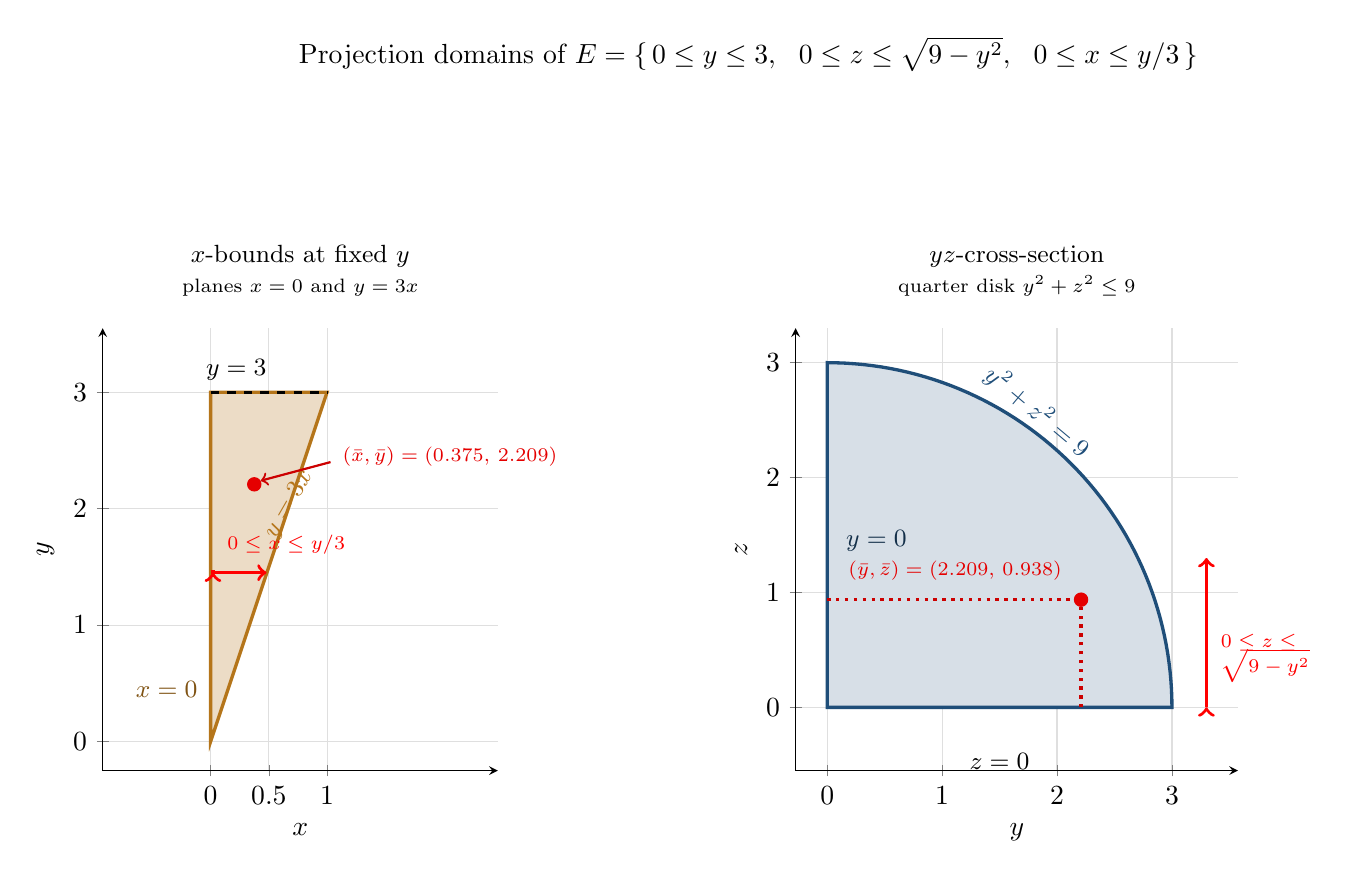
\begin{tikzpicture}
% ================= left: x-bounds at fixed y =================
\begin{scope}[shift={(0,0)}]
\begin{axis}[
    width=6.6cm, height=7.2cm, axis equal, axis lines=left, clip=false,
    xlabel=$x$, ylabel=$y$, xmin=-0.06,xmax=1.60, ymin=-0.25,ymax=3.55,
    xtick={0,0.5,1}, ytick={0,1,2,3}, grid=major, grid style={gray!25},
    title={$x$-bounds at fixed $y$\\ {\scriptsize planes $x=0$ and $y=3x$}},
    title style={font=\small\normalfont, align=center, yshift=2pt}]
    \addplot[fill=cbla!25, draw=cbla, very thick] coordinates {(0,0) (1,3) (0,3)} \closedcycle;
    \addplot[very thick, black, dashed, domain=0:1, samples=2] ({x},{3});
    \addplot[<->, red, very thick] (0.02,1.45) -- (0.48,1.45);
    \node[red, font=\scriptsize, anchor=south west] at (axis cs:0.06,1.52) {$0\le x\le y/3$};
    \node[cbla, font=\small, rotate=60, anchor=south west] at (axis cs:0.62,1.60) {$y=3x$};
    \node[cbla!70!black, font=\small, anchor=east] at (axis cs:-0.03,0.45) {$x=0$};
    \node[black, font=\small, anchor=south] at (axis cs:0.22,3.02) {$y=3$};
    \addplot[only marks, mark=*, mark size=2.4, red!90!black] coordinates {(0.3747,2.2089)};
    \node[red!90!black, font=\scriptsize, anchor=west, align=left] at (axis cs:1.05,2.45)
        {$(\bar x,\bar y)=(0.375,\,2.209)$};
    \draw[->, red!80!black, thick] (axis cs:1.03,2.40) -- (axis cs:0.43,2.24);
\end{axis}
\end{scope}
% ================= right: quarter disk in the yz-plane =================
\begin{scope}[shift={(8.8cm,0)}]
\begin{axis}[
    width=7.2cm, height=7.2cm, axis equal, axis lines=left, clip=false,
    xlabel=$y$, ylabel=$z$, xmin=-0.25,xmax=3.55, ymin=-0.55,ymax=3.3,
    xtick={0,1,2,3}, ytick={0,1,2,3}, grid=major, grid style={gray!25},
    title={$yz$-cross-section\\ {\scriptsize quarter disk $y^2+z^2\le 9$}},
    title style={font=\small\normalfont, align=center, yshift=2pt}]
    \addplot[fill=cblb!18, draw=cblb, very thick, domain=0:90, samples=61, variable=t]
        ({3*cos(t)},{3*sin(t)}) \closedcycle;
    \node[cblb, font=\small, rotate=-40, anchor=south] at (axis cs:1.70,2.42) {$y^2+z^2=9$};
    \node[black, font=\small, anchor=north] at (axis cs:1.5,-0.32) {$z=0$};
    \node[cblb!60!black, font=\small, anchor=west] at (axis cs:0.08,1.45) {$y=0$};
    \addplot[<->, red, very thick] (3.30,0) -- (3.30,1.30);
    \node[red, font=\scriptsize, anchor=north west, align=left] at (axis cs:3.34,0.72)
        {$0\le z\le$\\[-2pt] $\sqrt{9-y^2}$};
    \addplot[dotted, red!80!black, very thick] (2.2089,0) -- (2.2089,0.9375);
    \addplot[dotted, red!80!black, very thick] (0,0.9375) -- (2.2089,0.9375);
    \addplot[only marks, mark=*, mark size=2.4, red!90!black] coordinates {(2.2089,0.9375)};
    \node[red!90!black, font=\scriptsize, anchor=south west] at (axis cs:0.10,1.02)
        {$(\bar y,\bar z)=(2.209,\,0.938)$};
\end{axis}
\end{scope}
\node[font=\normalsize, align=center] at (8.2cm,9.1cm)
    {Projection domains of $E=\{\,0\le y\le 3,\ \ 0\le z\le\sqrt{9-y^2},\ \ 0\le x\le y/3\,\}$};
\end{tikzpicture}
\end{document}
